\documentclass[letterpaper]{article}


\PassOptionsToPackage{numbers}{natbib}
\usepackage[final]{neurips_2023}
\usepackage[utf8]{inputenc} % allow utf-8 input
\usepackage[T1]{fontenc}    % use 8-bit T1 fonts
\usepackage{hyperref}       % hyperlinks
\usepackage{url}            % simple URL typesetting
\usepackage{booktabs}       % professional-quality tables
\usepackage{amsfonts}       % blackboard math symbols
\usepackage{nicefrac}       % compact symbols for 1/2, etc.
\usepackage{microtype}      % microtypography
\usepackage{xcolor}         % colors
\usepackage{tikz}
\usepackage{pgfplots}
\usepackage{tabularx,ragged2e}


\newcolumntype{L}{>{\RaggedRight}X}
\pgfplotsset{width=10cm,compat=1.9}


%%%%%%%%%%%%%%%%%%%%%%%%%%%%%%%%%%%%%%%%%%%%%%%%%%%%%%%%%%%%


\title{GNN as Policy Network for Deep Reinforcement Learning Generalization}

\author{%
    Roozmehr Jalilian, Shidi Xi \\
    Department of Electrical \& Computer Engineering \\
    The University of British Columbia \\
    \texttt{\{roozmehr.jalilian,xsd99\}@ece.ubc.ca} \\
    Vancouver, BC V6T 1Z4
}


\begin{document}


\maketitle


\begin{abstract}
Routing in integrated circuits (IC) design is often modeled as a pathfinding problem and has consistently represented one of the most challenging aspects due to its complexity and time-consuming nature. Even with state-of-the-art commercial CAD tools, routing complex designs can take hours, if not days. Consequently, there is a growing interest in applying machine learning-based approaches to overcome these challenges. In previous work, we introduced a novel reinforcement learning (RL) approach for routing. While this RL router outperformed the baseline, it was limited by poor generalizability, requiring a new policy to be trained from scratch for each problem. In this project, we aim to address this limitation by introducing a novel graph neural network (GNN) as the policy network for the RL router. This enhancement allows the agents to generalize their learned routing policies to new, unseen designs, reducing the computation time significantly.
\end{abstract}

\section{Introduction}
IC routing involves connecting distinct electrical contact points (pins) on a chip using metallic wires. This process is crucial for the functionality of computer chips, as it enables data transfer and computing activities between components like the CPU and memory. We model routing as a pathfinding problem, representing the chip as a 2-dimensional grid. Pins, identified by their (x, y) coordinates, are placed on the grid's nodes. The objective is to establish paths connecting these nodes while navigating the grid edges. Each edge possesses a capacity feature, indicating the maximum number of permissible wires due to the physical constraints of wire thickness and finite space within a chip region. An optimal routing solution seeks to minimize total wire length and avoid edge overflow (usage of an edge exceeding its capacity), ensuring all connections are efficient and within capacity.

Two important terminologies here are net and netlist. A net refers to a set of pins requiring connection, and a netlist is a set comprises multiple nets needing routing during the process. And for clarity, we will use the terms nodes and pins interchangeably throughout this proposal.

In prior research, we introduced a multi-agent RL router to address the IC routing challenge. Each agent, tasked with routing one individual net, operated concurrently under a shared super policy, as we designed the agents to be homogeneous and fully-cooperative. Trained with proximal policy optimization (PPO) \cite{Schulman2017} and evaluated against benchmarks, this RL router demonstrated superior performance compared to the A* baseline. However, a limitation emerged: the policy, though effective for specific benchmarks, lacked generalizability for other, albeit similar, problems. We attributed this shortfall to the policy neural network's architecture, comprising several fully connected (FC) layers, which struggled to extract rich information from the state encodings.

Contrastingly, graph neural networks (GNNs) exhibit robust generalization capabilities when processing graphical data \cite{Almasan2022,Wang2018}, aligning with the routing problem’s grid graph model. In this project, we introduce a novel message-passing GNN architecture integrated into the RL router’s policy network. The GNN accepts the routing grid graph from the environment as state input and determines actions accordingly. This innovation aims to bolster the RL router’s ability to generalize trained policy to problems not encountered during training, promising substantial reductions in computation time.


%Digital logic design involves three major stages: {\bf RTL}\footnote{Register transfer level}{\bf design}, {\bf synthesis}, and {\bf physical design}. An engineer first decides on the architecture of a digital circuit, and describes it with the help of a {\it hardware description language} (HDL). The described architecture is then fed into a CAD tool, which first synthesizes the design using different logic gates, and then maps the gates onto the chip canvas.

%Physical design is perhaps the most challenging stage of the whole process, as it involves two sophisticated and time-consuming phases: {\bf placement} and {\bf routing}. The goal of this stage is to place a large number of logic gates on the chip and route them in such a way that the final circuit satisfies multiple constraints (timing, area, etc.). Routing, in general, is the more complex, as the wiring resources on the chip are limited and routing {\bf congestion} must also be taken into account.

%Due to the problem's complexity, routing is generally broken into two sub-phases: {\bf global} and {\bf detailed}. Global routing first partitions the chip into routing regions and searches for region-to-region paths for all signal nets; this is followed by detailed routing, which determines the exact tracks and vias of these nets based on their region assignments \cite{Kahng2022}.

%Obtaining a valid solution which satisfies all constraints might usually take up to several days for large circuits, leading to a surge of interest to use machine learning techniques, aiming to find solutions much faster while improving or maintaining the same level of solution quality.

%TODO: RL approach, poor generalizability, propose GNN as policy network, should probably trim down the wording for routing, as the focus for this project is about designing GNN to achieve RL generalizability.


\section{Related work}
Numerous studies in existing literature have verified the effectiveness of employing Graph Neural Networks (GNNs) within the policy/value network of Reinforcement Learning (RL) models to enhance generalization, especially when the agent’s environment is graph-representable. However, to our knowledge, no existing study has directly explored the use of GNN equipped RL for IC routing.

\cite{Liao2020} introduced an RL IC router trained via a Deep Q-Network (DQN), utilizing a multi-layer perceptron (MLP) as the RL agent's value network. However, similar to our previous work, it showed a lack of generalization. Contrastingly, \cite{Almasan2022} incorporated a GNN as the value network of an RL agent, also trained by DQN. This approach manifested notable generalization capabilities in network routing—a field bearing similarities to IC routing—and serves as the principal inspiration for our current proposal. In parallel, both \cite{Chen2023} and \cite{Wang2018} echoed the integration of GNNs with RL models wherein the operational problems are graphs. Furthermore, \cite{Mirhoseini2021} and \cite{Yue2022} adopted GNNs as encoder layers for their respective RL policy and value networks.

    
\section{Methodology}
In this proposal, we limit our discussion to a simplified case of IC routing to facilitate the rapid development of a prototype. As the project advances, we will introduce additional complexities to refine and compact the model.

\subsection{Modeling IC routing as a grid graph}
\autoref{fig:grid} illustrates a simplified IC routing problem, represented as a grid graph with a single net. The grid, sized 4x4 and with an edge capacity of 1, contains a net composed of two pins positioned at coordinates (0,0) and (3,3). The grid comprises 16 nodes in total. Assuming the RL agent initiates its path at node (0,0), its destination is fixed at (3,3). The grid is defined by a node feature matrix $\mathbf{X}$, an edge feature matrix $\mathbf{E}$, and the adjacency matrix $\mathbf{A}$.

Matrix $\mathbf{X}$, with dimensions of 16x2, consists of rows that represent the binary feature vectors of nodes. The first element of each row signifies the presence of the RL agent, while the second element indicates whether a target resides at that specific node. Both $\mathbf{E}$ and $\mathbf{A}$ are 16x16 matrices. In particular, $\mathbf{E}$ encapsulates the scalar capacities of the edges connecting the nodes.


\begin{figure}[h!]
    \centering
    \includegraphics[width=0.3\textwidth]{figure/grid_grap.png}
    \caption{The grid graph of a simple IC routing problem.}
    \label{fig:grid}
\end{figure}

\subsection{GNN architectural design}
The GNN employs a message-passing mechanism, processing inputs of matrices $\mathbf{X}$, $\mathbf{E}$, and $\mathbf{A}$ from the RL environment and yielding the probability distribution of all potential actions. An MLP implements the message network, with messages being aggregated through element-wise summation. Node states are updated using a Gated Recurrent Unit (GRU). 

Following the message-passing phase, the updated node states are fed into another MLP, culminating in a softmax layer that generates the action probability distribution.

The GNN architecture cannot reply on the graph topology, e.g., the number of nodes. We want the GNN to generalize to graphs of any size. 

\subsection{RL policy training}
We plan to integrate the proposed GNN into our RL router, serving as its policy network. The training will be conducted using PPO with RLlib. The GNN's parameters will be refined through stochastic gradient descent, guided by feedback from the value network.


%TODO: Briefly explain what is multi-agent RL and its advantages for our given problem. Also mention the paper which used a GNN as the policy network for the RL agent \cite{Almasan2022}. Also discuss the overall architecture of the GNN that we're going to use, and mention which libraries we're using (i.e., PyTorch, PyG, and RLLib). Adding a figure depicting the routing problem in a grid would also be very helpful. Also, don't forget to come up with a rough timeline and replace the 'X' values below!

\subsection{Project Timeline}
\begin{itemize}
    \item Conduct an extended literature review to gather comprehensive insights and foundational knowledge (5 days).
    \item Develop the GNN prototype, integrate it with the RL router, and initiate training on a preliminary benchmark (14 days).
    \item Evaluate the enhanced RL router’s performance on a variety of benchmarks, including those analogous and distinct from the training set (1 day).
    \item Analyze the outcomes to assess the model's generalization capabilities and performance metrics, making figures and tables (3 days).
    \item (Bonus) Expand the model and its design to accommodate multi-agent concurrent routing, enhancing scalability and efficiency (7 days).
    \item Writing up the report (14 days).
\end{itemize}

    
\section{Experiments}
We will construct a baseline using an MLP policy network and train it on a simple benchmark to facilitate a comparative analysis.

\subsection{Comparing Training Efficiency}
This experiment aims to compare the training efficiency of the GNN-equipped router with the baseline router, both trained on the same benchmark. We will assess their performance by examining the plots of reward versus training iterations. The objective is to evaluate the training efficiency of the GNN-equipped router in comparison to the baseline. As suggested by \cite{Wang2018}, we anticipate that the new design will demonstrate comparable, if not superior, training efficiency.

\subsection{Comparing Zero-Shot Performance} \label{m:0}
We will employ the zero-shot policies derived from the previous experiment to perform inference on several unseen benchmarks. These benchmarks will feature netlists with canvas sizes, numbers of nets, and total numbers of pins per net that resemble the training benchmark. The comparison criteria will include rewards and routing solution quality (wire length, overflow). We predict that the new GNN-equipped design will surpass the baseline in performance.

\subsection{Comparing Fine-Tuning Performance}
This experiment is designed to evaluate the scalability of the GNN to more complex problems. We will initiate zero-shot inference on benchmarks characterized by different numbers of nets, chip canvas sizes, and numbers of pins per net than the training benchmark. We anticipate a decrease in zero-shot performance compared to the results of \autoref{m:0}, indicating a likely need for policy fine-tuning.

Both the new design and baseline policies will undergo fine-tuning for an equal number of iterations. We will compare their performances based on rewards and solution quality metrics. Our expectation leans towards the new GNN-equipped design demonstrating superior adaptability and performance after fine-tuning.

\begin{figure}[h!]
    \centering
    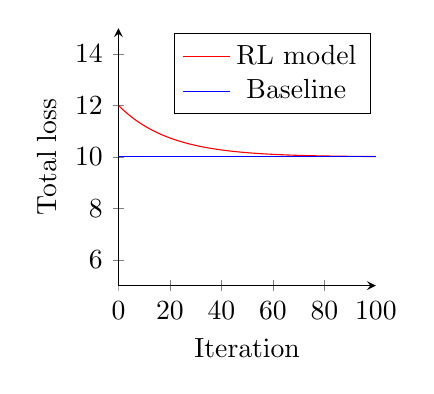
\begin{tikzpicture}
        \begin{axis}[
            width=0.4\textwidth,
            height=0.4\textwidth, 
            axis lines = left,
            xlabel = Iteration,
            ylabel = Total loss,
            ymin=5, ymax=15,
            ]
            % The reward function
            \addplot [
            domain=0:100, 
            samples=100, 
            color=red,
            ]
            {10 + 2 * exp(-x / 20)};
            \addlegendentry{RL model}
            % Baseline
            \addplot [
            domain=0:100, 
            samples=100, 
            color=blue,
            ]
            {10};
            \addlegendentry{Baseline}
        \end{axis}
    \end{tikzpicture}
    \caption{Placeholder figure for total loss vs. time. Not related to any aforementioned experiments.}
\end{figure}

\begin{table}[h!]
    \caption{Placeholder table for the experiments. Not related to any aforementioned experiments.}
    \centering
    \begin{tabularx}{\textwidth}{LLLLLLL}
        \toprule
        \multicolumn{4}{c}{Benchmark specs} &
        \multicolumn{3}{c}{Results} \\
        \cmidrule(r){1-4}
        \cmidrule(r){5-7}
        Name & Canvas size & \# of nets & Avg. \# of pins per net & Runtime (s) & Max. memory usage (MB) & Total wirelength \\
        \midrule
        test1 & \(8 \times 8\) & 5 & 2.5 & 1.25 & 250 & 100 \\
        test2 & \(6 \times 6\) & 3 & 1 & 0.60 & 150 & 70 \\
        \bottomrule
    \end{tabularx}
\end{table}
    
%%%%%%%%%%%%%%%%%%%%%%%%%%%%%%%%%%%%%%%%%%%%%%%%%%%%%%%%%%%%
    
{
\small
\bibliographystyle{IEEEtranN}
\bibliography{references}
}

%%%%%%%%%%%%%%%%%%%%%%%%%%%%%%%%%%%%%%%%%%%%%%%%%%%%%%%%%%%%


\end{document}